\documentclass{beamer}
\usepackage{algorithm}
\usepackage{algpseudocode}
\usepackage{caption}
\usepackage{hyperref}
\renewcommand\vec[1]{\ifstrequal{#1}{0}{\ensuremath{\mathbf{0}}}{\ensuremath{\boldsymbol{#1}}}}
\setbeamertemplate{headline}{}


\usetheme[compress]{Berlin}
\setbeamertemplate{page number in head/foot}[framenumber]
\captionsetup{justification=centering, font={scriptsize}, skip=0pt}

\title[Dinámica Molecular Dirigida Por Eventos]{Dinámica Molecular Dirigida por Eventos: Trabajo Práctico N°3}
\subtitle{72.25 - Simulación de Sistemas}
\author[M. Barnatán, I. Maruottolo Quiroga, I. Pedemonte Berthoud]{
  Martín Alejandro Barnatán\inst{1} \and 
  Ignacio Martín Maruottolo Quiroga\inst{2} \and 
  Ignacio Pedemonte Berthoud\inst{3}
}
\institute[ITBA]{
  \inst{1} mbarnatan@itba.edu.ar (64463) \\
  \inst{2} imaruottoloquiroga@itba.edu.ar (64611) \\
  \inst{3} ipedemonteberthoud@itba.edu.ar (64908) \\
}
\date{2025 2C | Grupo Nº10}
\titlegraphic{
\includegraphics[height=1.2cm]{resources/itba.png}}

\makeatletter
\beamer@theme@subsectionfalse
\makeatother

\AtBeginSection[]{
    \begin{frame}
        \begin{beamercolorbox}[sep=8pt,center]{title}
            \usebeamerfont{title}\insertsection
        \end{beamercolorbox}
    \end{frame}
}

\begin{document}

\begin{frame}
  \titlepage
\end{frame}

% Sección 1
\section{Introducción}
\begin{frame}{Sistema Real}
Estudio de un sistema de $N$ partículas con radio $R$ y velocidad inicial $v$, 
que colisionan entre sí y contra las paredes del contenedor. 
  \begin{columns}[T,onlytextwidth]
    \begin{column}{0.50\textwidth}
    \begin{itemize}
      \item Difusión de un gas.
      \item Efusión (Knudsen): tasa de fuga.
      \item Cuello de botella: caudal/atascos.
    \end{itemize}
    \end{column}
    \hfill
    \begin{column}{0.40\textwidth}
      \centering
      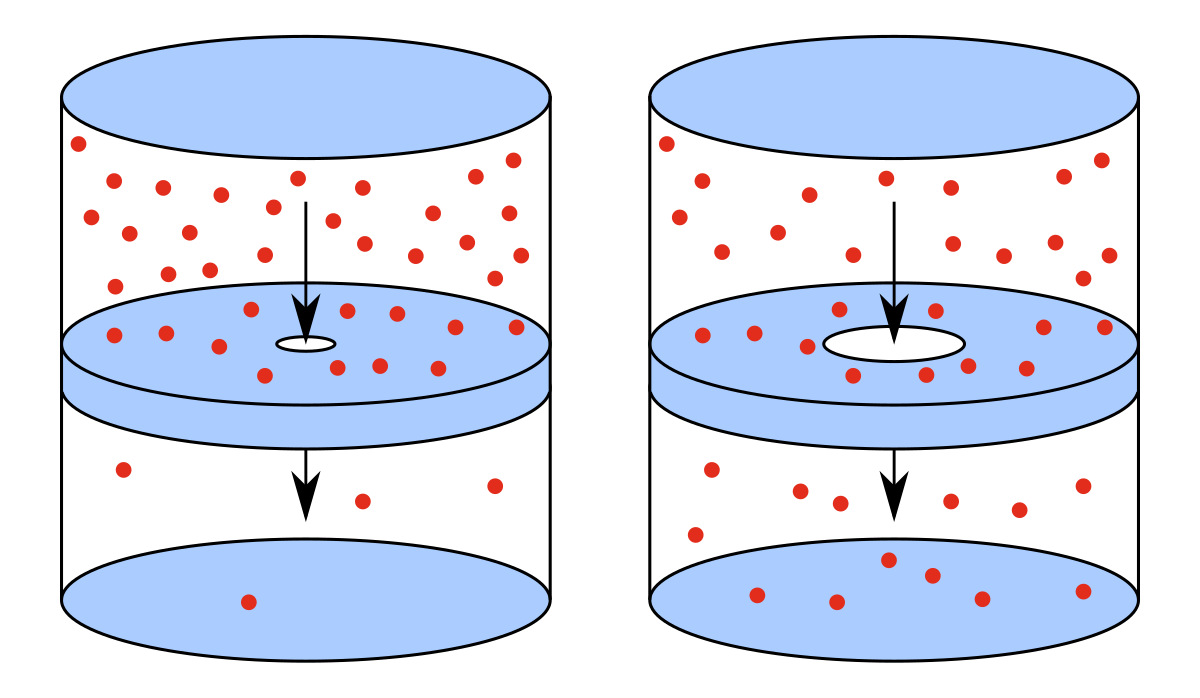
\includegraphics[width=\linewidth]{resources/efusion.png}
    \end{column}
  \end{columns}
\end{frame}


\begin{frame}{Fundamentos}
    Las partículas actualizan su posición mediante:
    \begin{equation*}
        x_i(t_c) = x_i(t) + v_{x_i}t_c
    \end{equation*}
    \begin{equation*}
        y_i(t_c) = y_i(t) + v_{y_i}t_c
    \end{equation*}
    Donde $t_c$ es el tiempo de choque y se define:
    \begin{equation*} 
        t_c=
        \left\{
        \begin{array}{ll}
        \infty & \text{si } \vec{\Delta v}\cdot\vec{\Delta r}\ge0,\\
        \infty & \text{si } d<0,\\
        -\frac{\vec{\Delta v}\cdot\vec{\Delta r}+\sqrt{d}}{\vec{\Delta v}\cdot\vec{\Delta v}}  & \text{en otro caso}
        \end{array}
        \right. 
    \end{equation*}
    \begin{itemize}
        \item $\vec{\Delta r}$: vector de posiciones relativas
        \item $\vec{\Delta v}$: vector de velocidades relativas
        \item $d$: discriminante de la cuadrática en la condición de choque
    \end{itemize}
\end{frame}

\begin{frame}{Fundamentos}
    En el choque entre dos partículas, el impulso se calcula mediante: 
    \begin{equation*}
        J_x=\frac{J\Delta x}{\sigma}, J_y=\frac{J\Delta y}{\sigma}
    \end{equation*}
    \begin{equation*}
        J=\frac{2m_im_j(\vec{\Delta v}\cdot\vec{\Delta r})}{\sigma(m_i+m_j)}
    \end{equation*}
    Donde $m_i$, $m_j$ son las masas de las partículas y $\sigma=R_i+R_j$.\\
    Las velocidades luego se actualizan según:
    \begin{columns}[T,onlytextwidth]
        \begin{column}{0.50\textwidth}
            \begin{equation*}
                vx_i^d=vx_i^a+\frac{J_x}{m_i}
            \end{equation*}
            \begin{equation*}
                vy_i^d=vy_i^a+\frac{J_y}{m_i}
            \end{equation*}
        \end{column}
        \begin{column}{0.50\textwidth}
            \begin{equation*}
                vx_j^d=vx_j^a-\frac{J_x}{m_j}
            \end{equation*}
            \begin{equation*}
                vy_j^d=vy_j^a-\frac{J_y}{m_j}
            \end{equation*}
        \end{column}
    \end{columns}
\end{frame}

% Sección 2
\section{Implementación}

\begin{frame}{Diagrama UML}
    \begin{figure}[htbp]
        \centering
        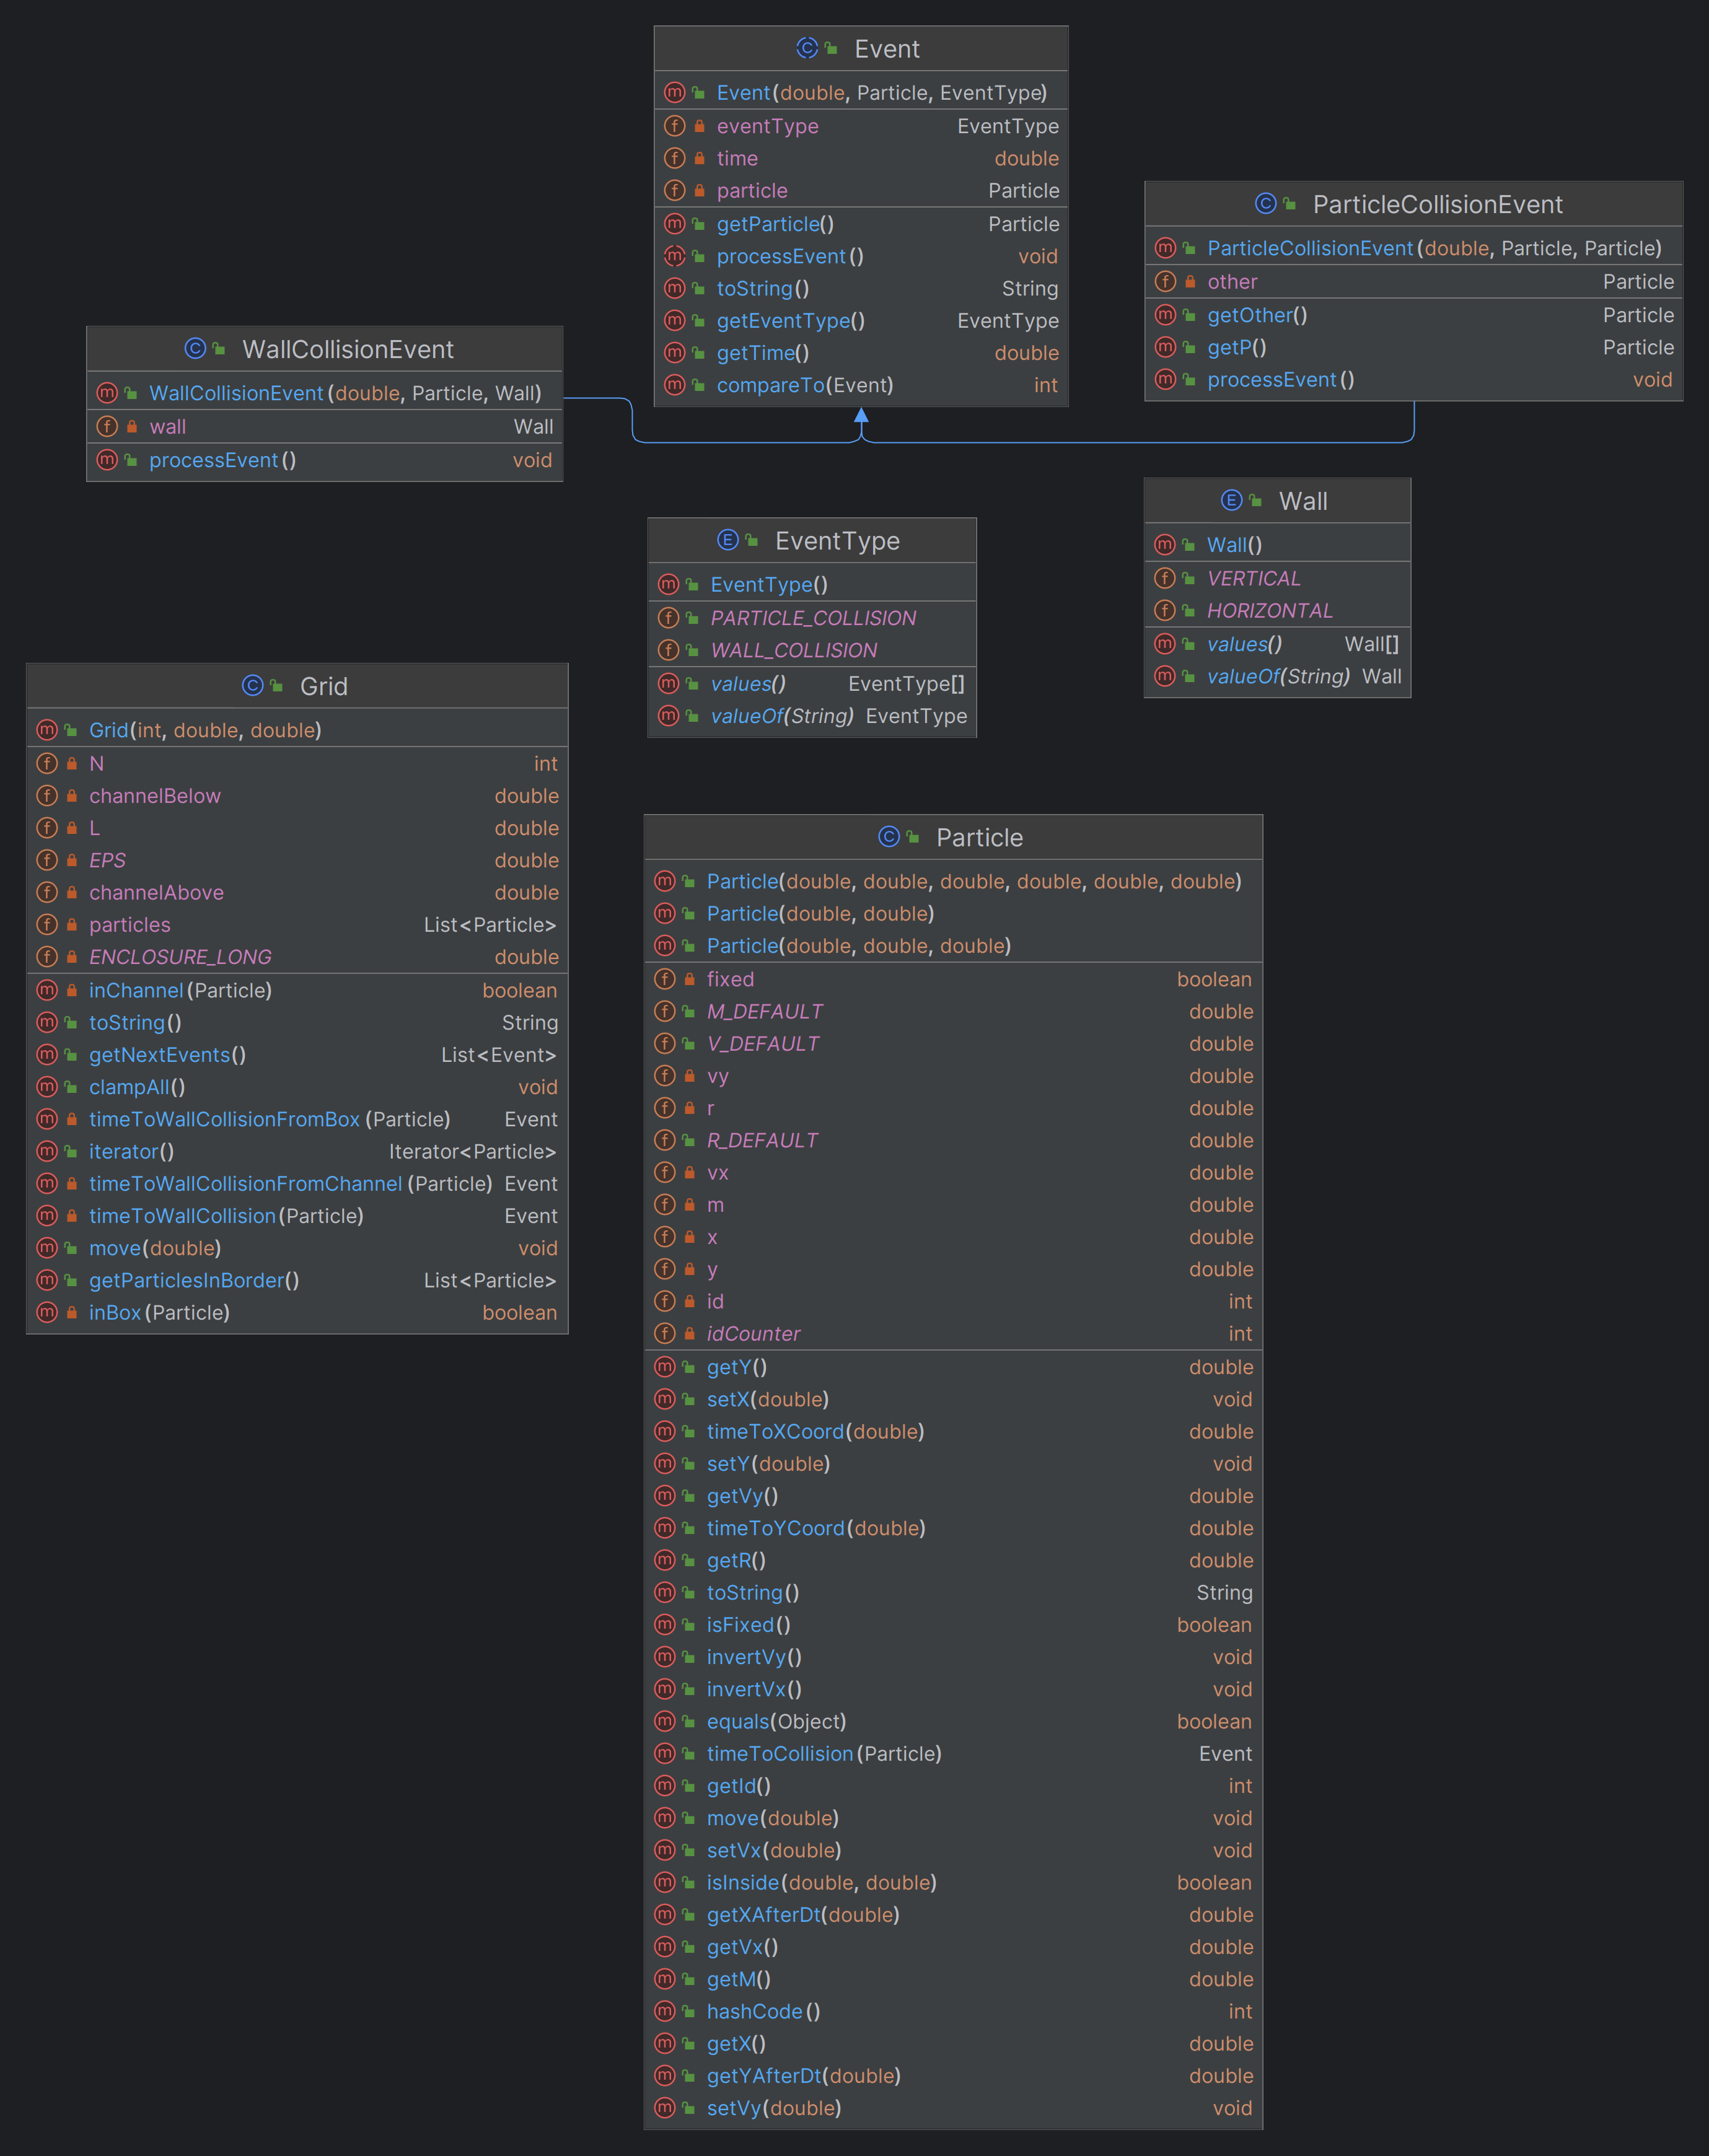
\includegraphics[width=0.45\textwidth]{resources/diagrama.png}
    \end{figure}
\end{frame}

\begin{frame}{Algoritmo Implementado}
    \begin{figure}[htbp]
        \centering
        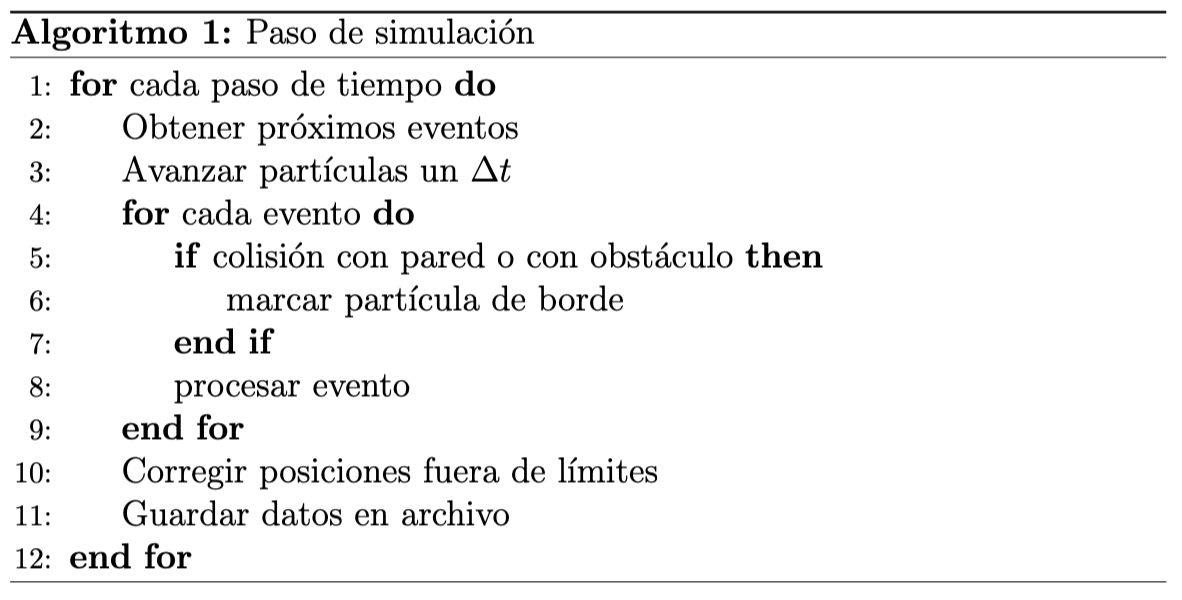
\includegraphics[width=0.9\textwidth]{resources/algorithm.png}
    \end{figure}
\end{frame}

% Sección 3
\section{Simulaciones}

\begin{frame}{Sistema Estudiado}
    \begin{figure}[htbp]
        \centering
        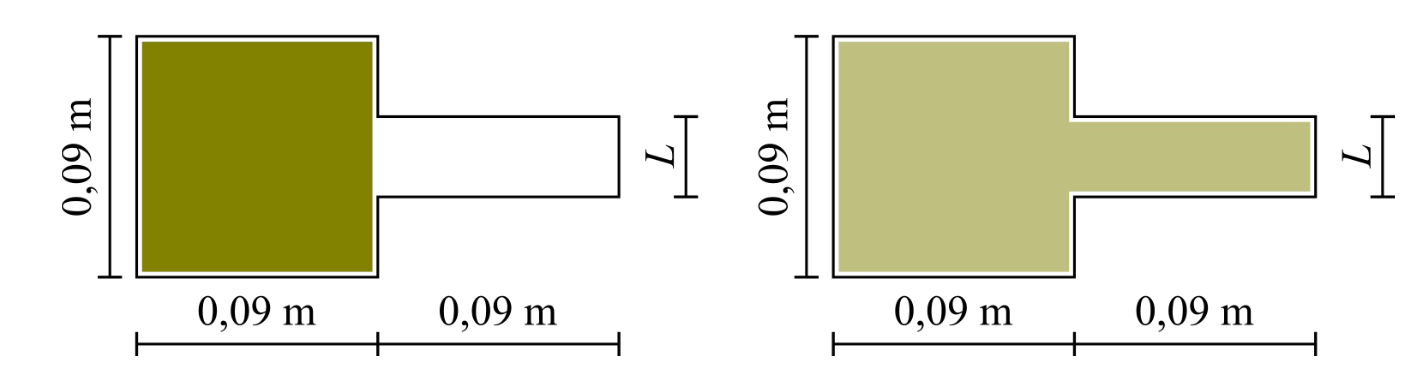
\includegraphics[width=0.9\textwidth]{resources/system.png}
    \end{figure}
\end{frame}

\begin{frame}{Colisión con Esquinas}
    \begin{columns}[c]
        \column{0.55\textwidth}
            \begin{itemize}
                \item Se ubica un obstáculo en el vértice.
                \item El obstáculo no tiene radio.
                \item Se calcula la matriz de colisión con restitución elástica perfecta.
            \end{itemize}
        \column{0.50\textwidth}
            \centering
            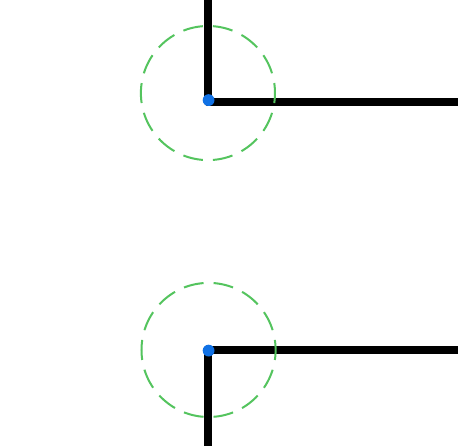
\includegraphics[width=\linewidth]{resources/bordes.png}
    \end{columns}
\end{frame}

\begin{frame}{Simulaciones}
    Parámetros de entrada fijos:
    \begin{itemize}
        \item $R=0.0015$m - Radio de Interacción
        \item $v=0.01$m/s - Módulo de la Velocidad
        \item $m=1$kg - Masa
        \item $T=30\,000$ - Eventos
        \item $N=300$ - Cantidad de Partículas
    \end{itemize}
    Parámetros de entrada variables:
    \begin{itemize}
        \item $L\in[0.03, 0.09]$m - Longitud del Lado del Canal
    \end{itemize}
\end{frame}

\begin{frame}{Cálculo de la Presión}
    La presión $P$ se calcula:
    \begin{equation*}
        P=\frac{\sum_{i\in C}\Delta p_i}{\Delta t \cdot L_T}
    \end{equation*}
    Donde $C$ es el conjunto de las colisiones ocurridas en $\Delta t$ y:
    \begin{itemize}
        \item $\Delta p_i=2m|v_{n,i}|$
        \item $L_T$ - Sumatoria de las paredes del recinto tomado
        \begin{itemize}
            \item $L_{T_i}=4\cdot(0.09m)-L$
            \item $L_{T_d}=2\cdot(0.09m)-L$
        \end{itemize}
    \end{itemize}
\end{frame}

\begin{frame}{Coeficiente de Difusión}
    El desplazamiento cuadrático medio se calcula:
    \begin{equation*}
        MSD(t)=\frac{1}{N}\sum_{i=1}^{N} \left| \vec{r}_i(t) - \vec{r}_i(t_0) \right|^2
    \end{equation*}
    Donde $\vec{r}_i(t)$ es la posición de la partícula $i$ en el tiempo $t$, y $t_0$ el tiempo de referencia. Luego:
    \begin{equation*}
        D=\frac{a}{2d}
    \end{equation*}
    Donde $a$ es la tasa promedio de crecimiento del desplazamiento cuadrático medio con el tiempo.
\end{frame}

% Sección 4
\section{Resultados}
\begin{frame}{Sistema con $L=0.03$m}{Animación}
    \begin{figure}[H!]
        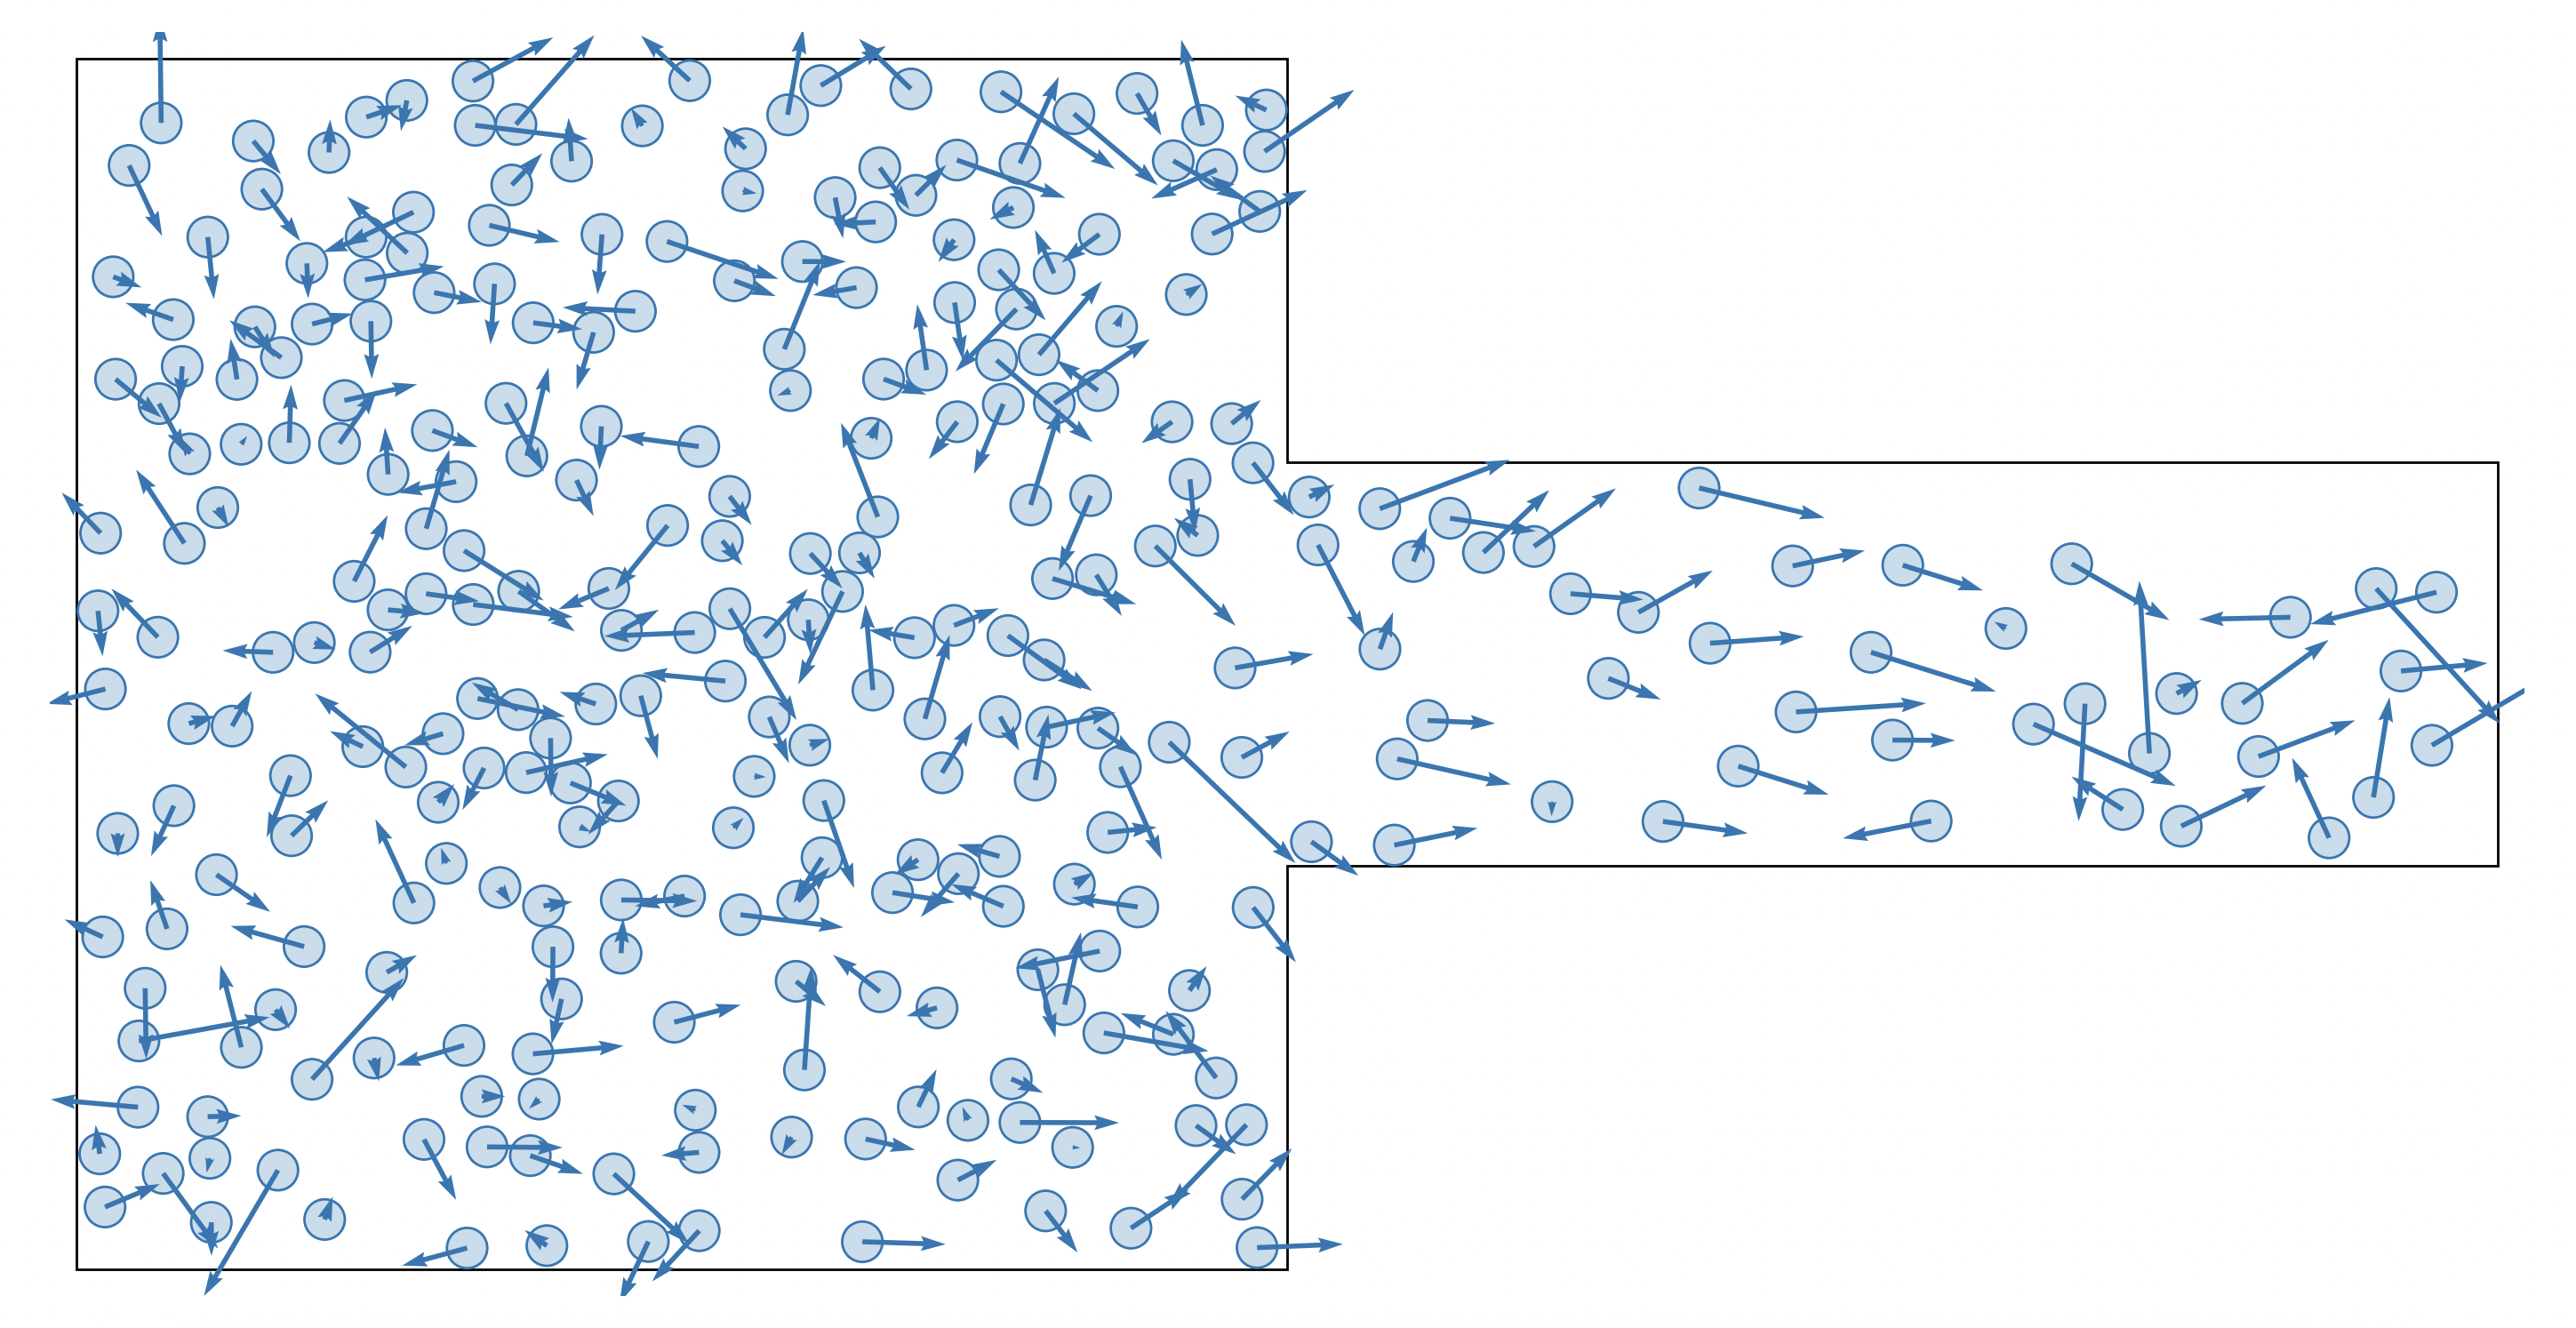
\includegraphics[height=.50\textheight]{resources/animacion-L003.png}
        \caption*{\href{https://youtu.be/mwGB-1hMv7Y}{Animación completa en https://youtu.be/mwGB-1hMv7Y}}
        \label{animacion-eta-0.1}
    \end{figure}
    \begin{beamercolorbox}[sep=5pt,center]{block body}
        \begin{minipage}[t]{0.3\textwidth}
            \centering
            \small{$N=300$}
        \end{minipage}
        \hfill
        \begin{minipage}[t]{0.3\textwidth}
            \centering
            \small{$T=30\,000$}
        \end{minipage}
        \hfill
        \begin{minipage}[t]{0.3\textwidth}
            \centering
            \small{$L = 0.03$m}
        \end{minipage}
    \end{beamercolorbox}
\end{frame}

\begin{frame}{Presión para $L=0.03$m}{Observable: Presión}
    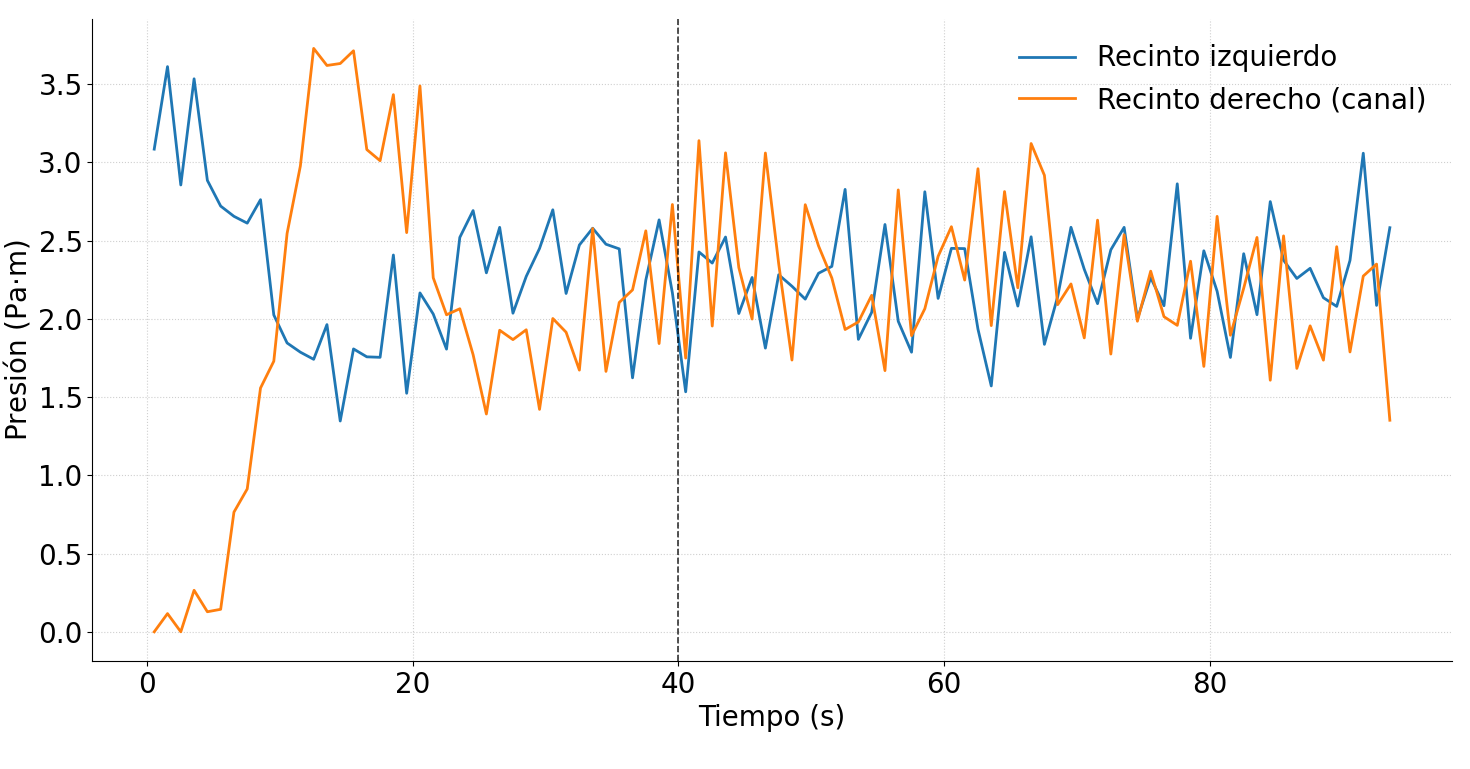
\includegraphics[width=\linewidth]{resources/presion-recintos-L003.png}
    \begin{beamercolorbox}[sep=5pt,center]{block body}
        \begin{minipage}[t]{0.3\textwidth}
            \centering
            \small{$N=300$}
        \end{minipage}
        \hfill
        \begin{minipage}[t]{0.3\textwidth}
            \centering
            \small{$T=30\,000$}
        \end{minipage}
        \hfill
        \begin{minipage}[t]{0.3\textwidth}
            \centering
            \small{$L = 0.03$m}
        \end{minipage}
    \end{beamercolorbox}
\end{frame}

\begin{frame}{Sistema con $L=0.09$m}{Animación}
    \begin{figure}[H!]
        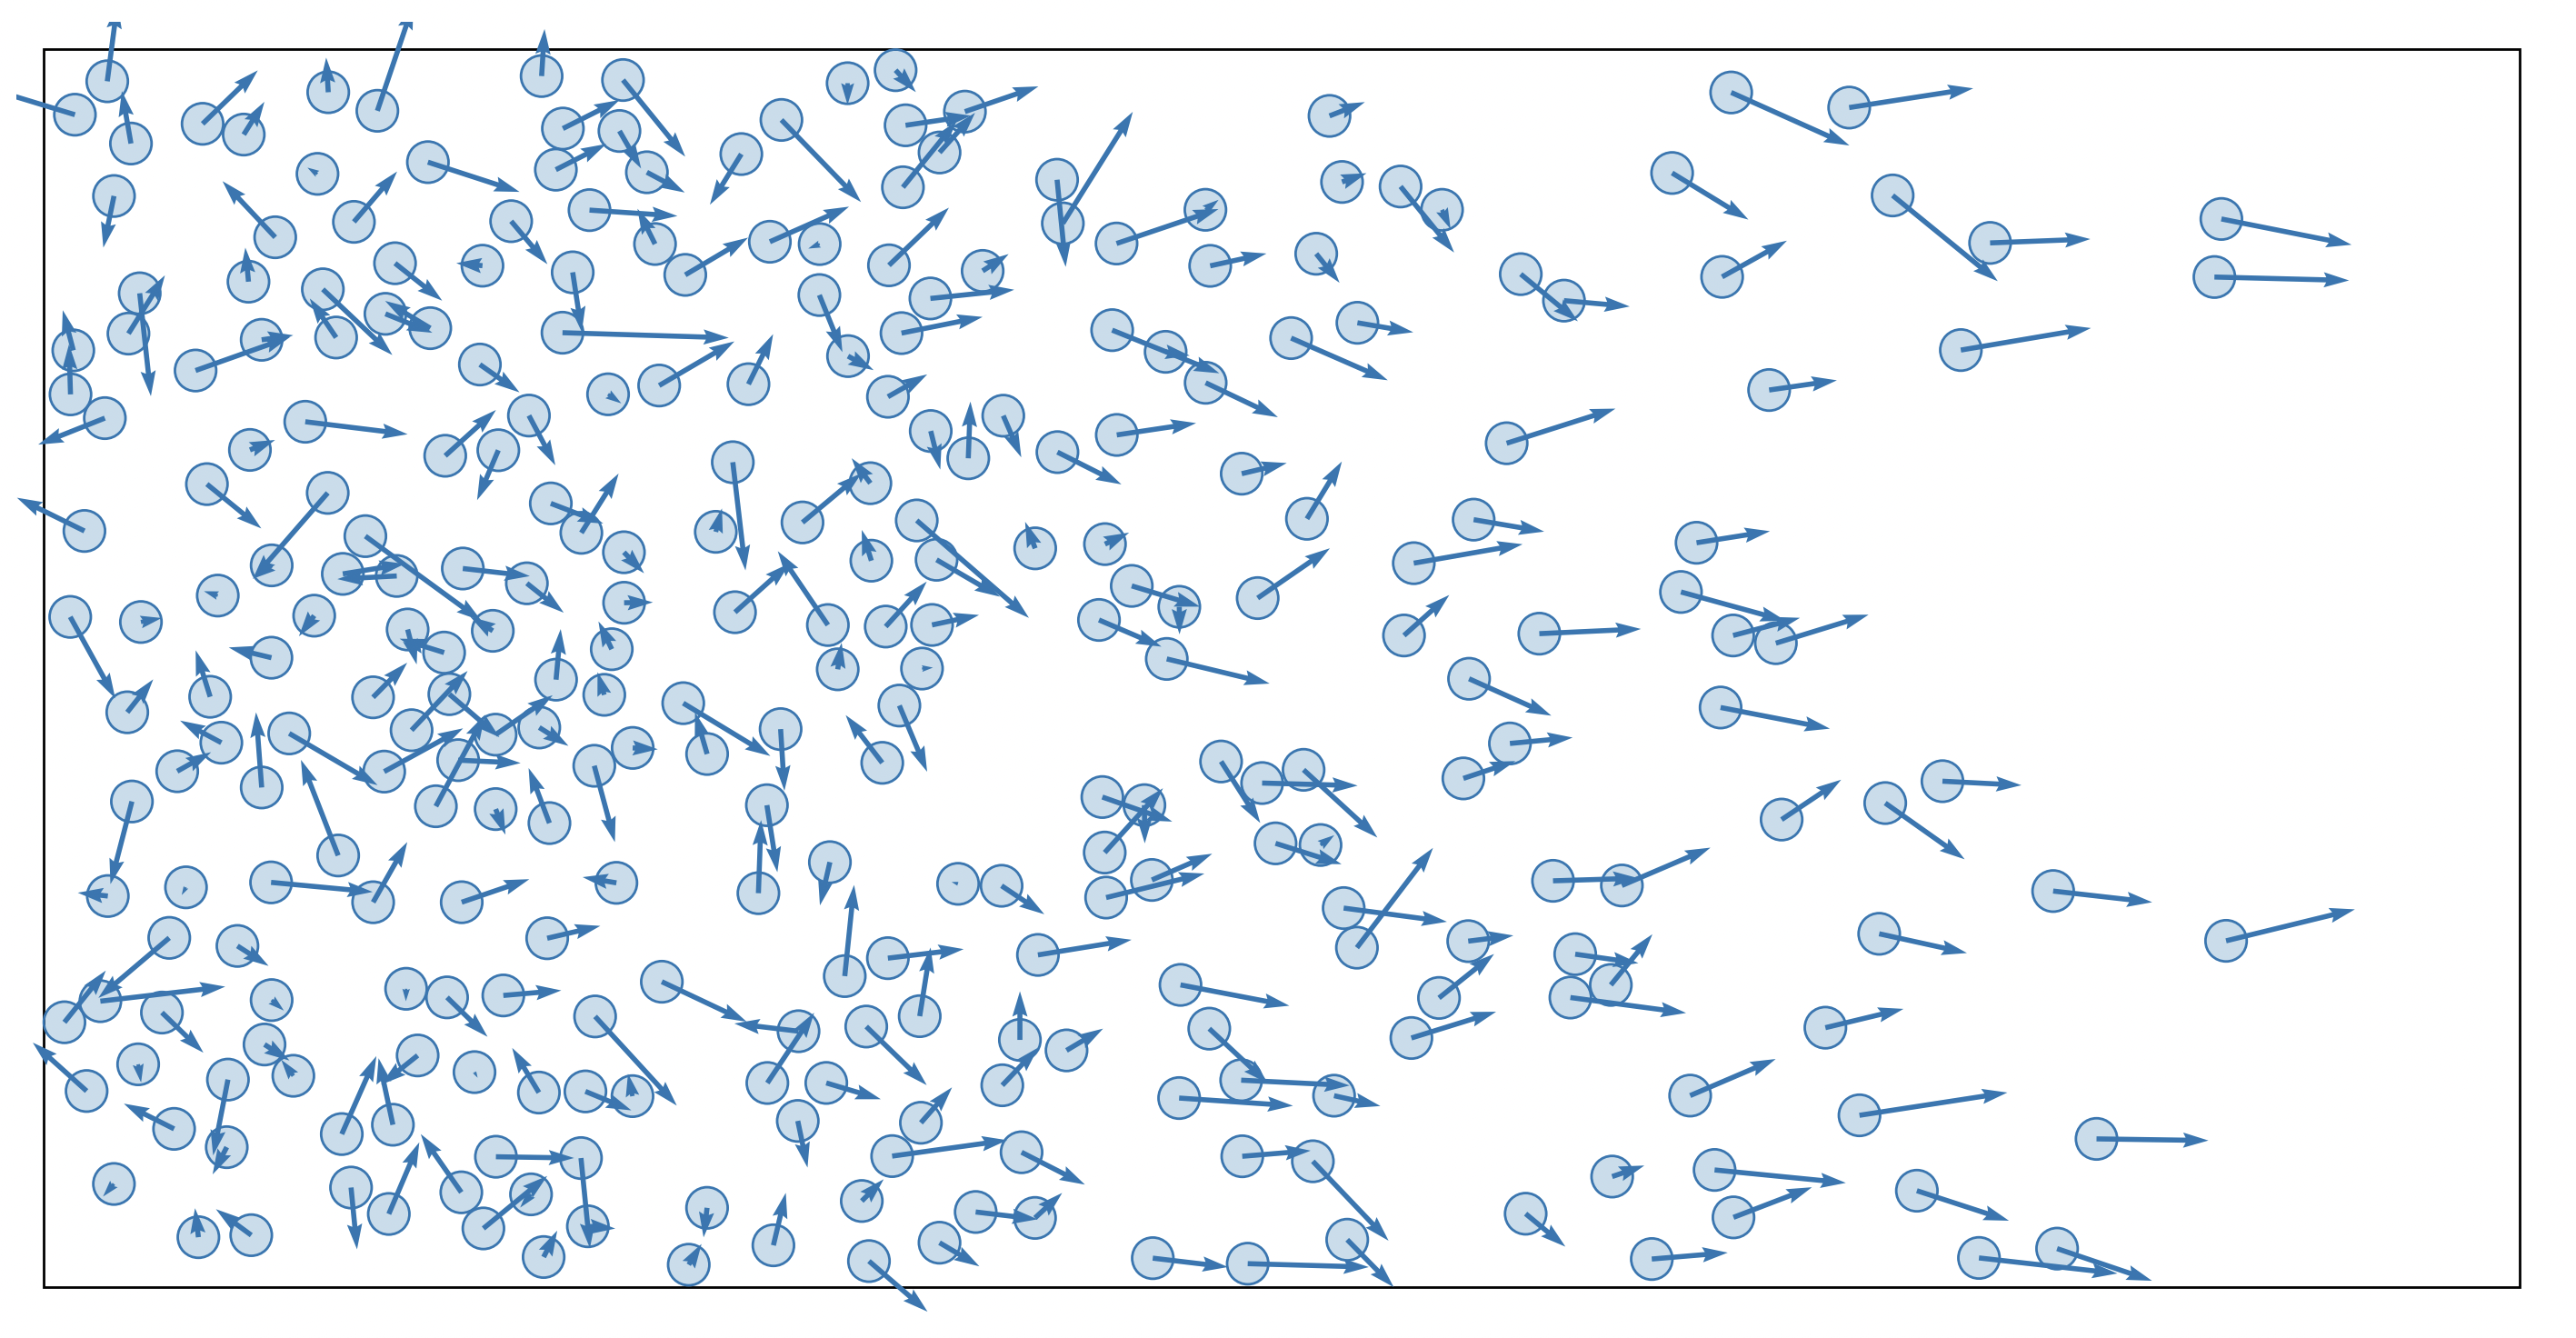
\includegraphics[height=.50\textheight]{resources/animacion-L009.png}
        \caption*{\href{https://youtu.be/kezvPD0NLVQ}{Animación completa en https://youtu.be/kezvPD0NLVQ}}
    \end{figure}
    \begin{beamercolorbox}[sep=5pt,center]{block body}
        \begin{minipage}[t]{0.3\textwidth}
            \centering
            \small{$N=300$}
        \end{minipage}
        \hfill
        \begin{minipage}[t]{0.3\textwidth}
            \centering
            \small{$T=30\,000$}
        \end{minipage}
        \hfill
        \begin{minipage}[t]{0.3\textwidth}
            \centering
            \small{$L = 0.09$m}
        \end{minipage}
    \end{beamercolorbox}
\end{frame}

\begin{frame}{Presión para $L=0.09$m}{Observable: Presión}
    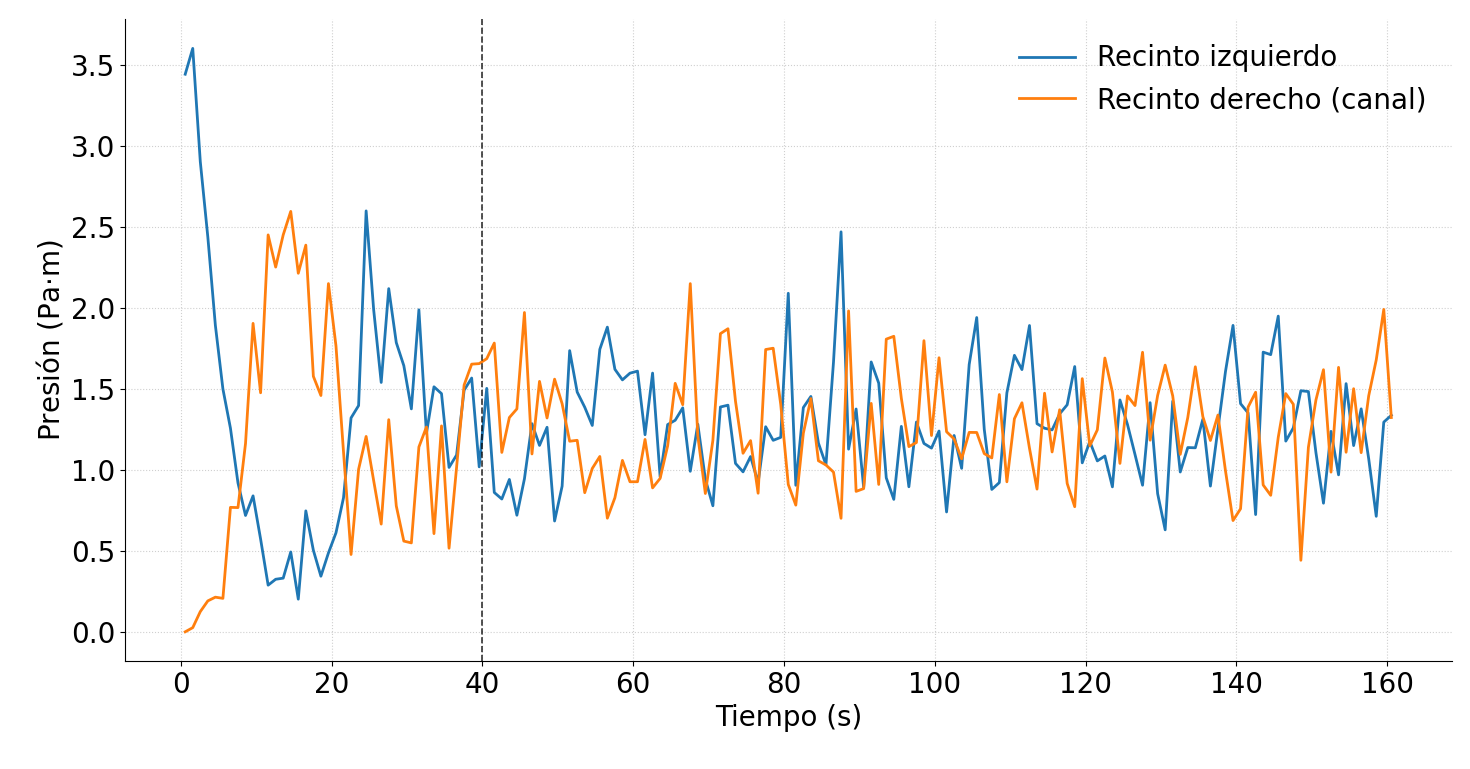
\includegraphics[width=\linewidth]{resources/presion-recintos-L009.png}
    \begin{beamercolorbox}[sep=5pt,center]{block body}
        \begin{minipage}[t]{0.3\textwidth}
            \centering
            \small{$N=300$}
        \end{minipage}
        \hfill
        \begin{minipage}[t]{0.3\textwidth}
            \centering
            \small{$T=30\,000$}
        \end{minipage}
        \hfill
        \begin{minipage}[t]{0.3\textwidth}
            \centering
            \small{$L = 0.09$m}
        \end{minipage}
    \end{beamercolorbox}
\end{frame}

\begin{frame}{Curva de Presión vs Área$^{-1}$}{En Régimen Estacionario}  
    \centering
    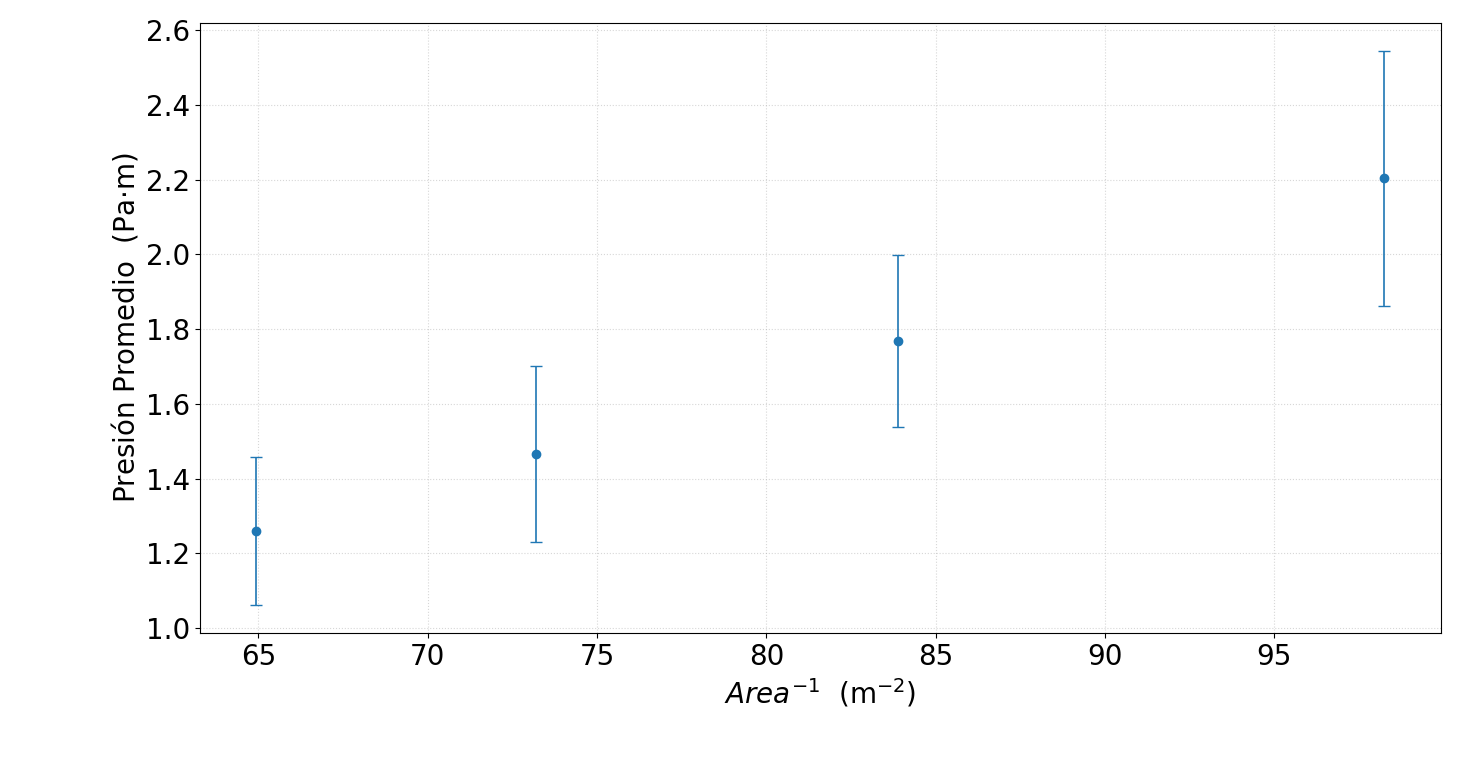
\includegraphics[width=\linewidth]{resources/presion-area.png}
    \begin{beamercolorbox}[sep=5pt,center]{block body}
        \begin{minipage}[t]{0.3\textwidth}
            \centering
            \small{$N=300$}
        \end{minipage}
        \hfill
        \begin{minipage}[t]{0.3\textwidth}
            \centering
            \small{$T=30\,000$}
        \end{minipage}
    \end{beamercolorbox}
\end{frame}

\begin{frame}{Ajuste Para el Modelo $P\sim A^{-1}$}{En Régimen Estacionario}
    \begin{columns}[c]
        \column{0.48\textwidth}
            \centering
            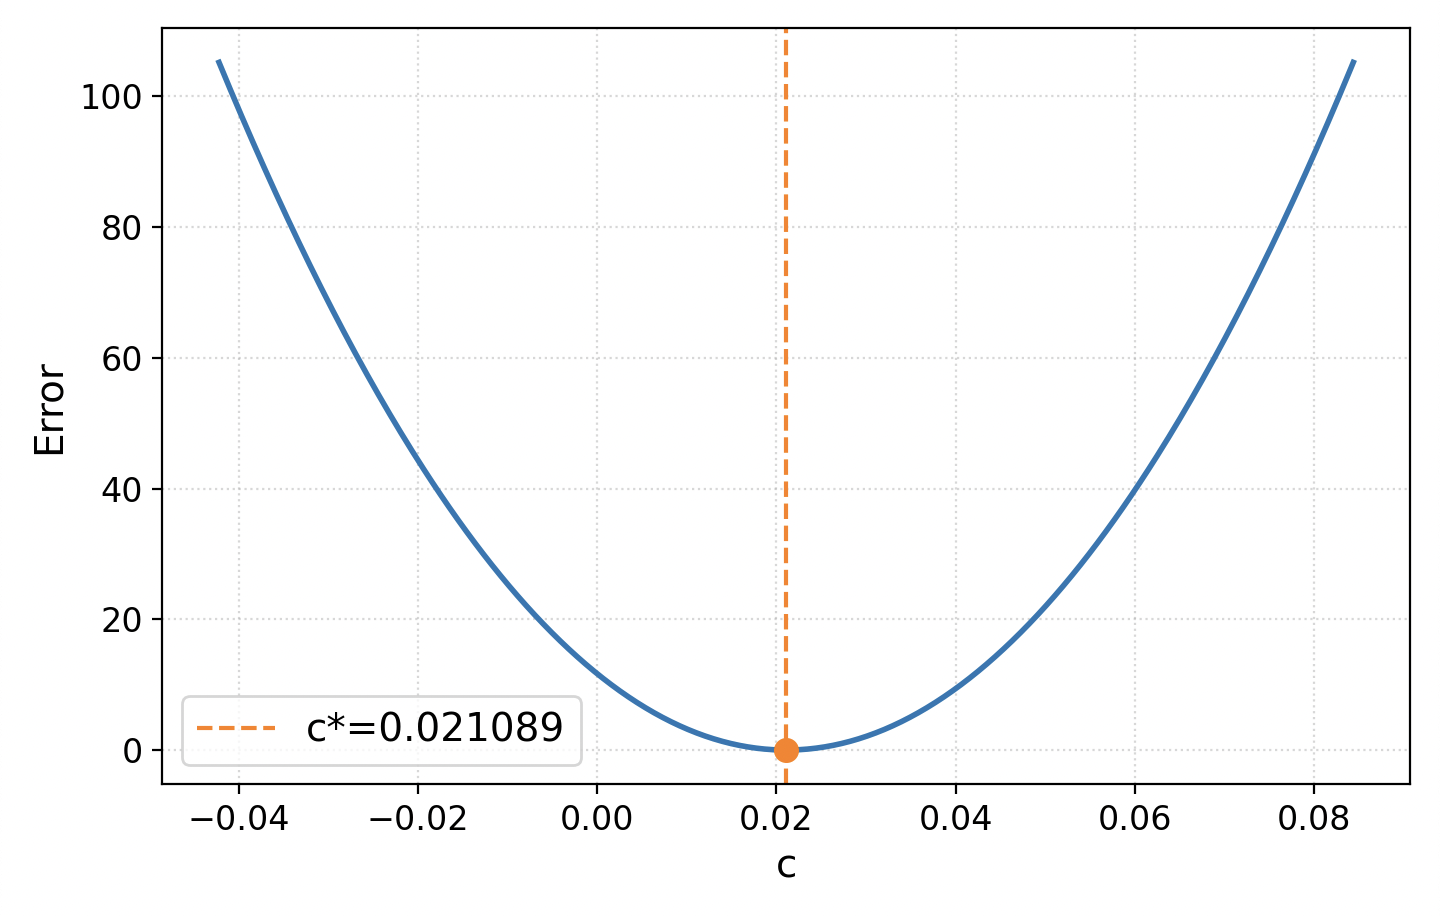
\includegraphics[width=\linewidth]{resources/error-regresion.png}
        \column{0.48\textwidth}
            \centering
            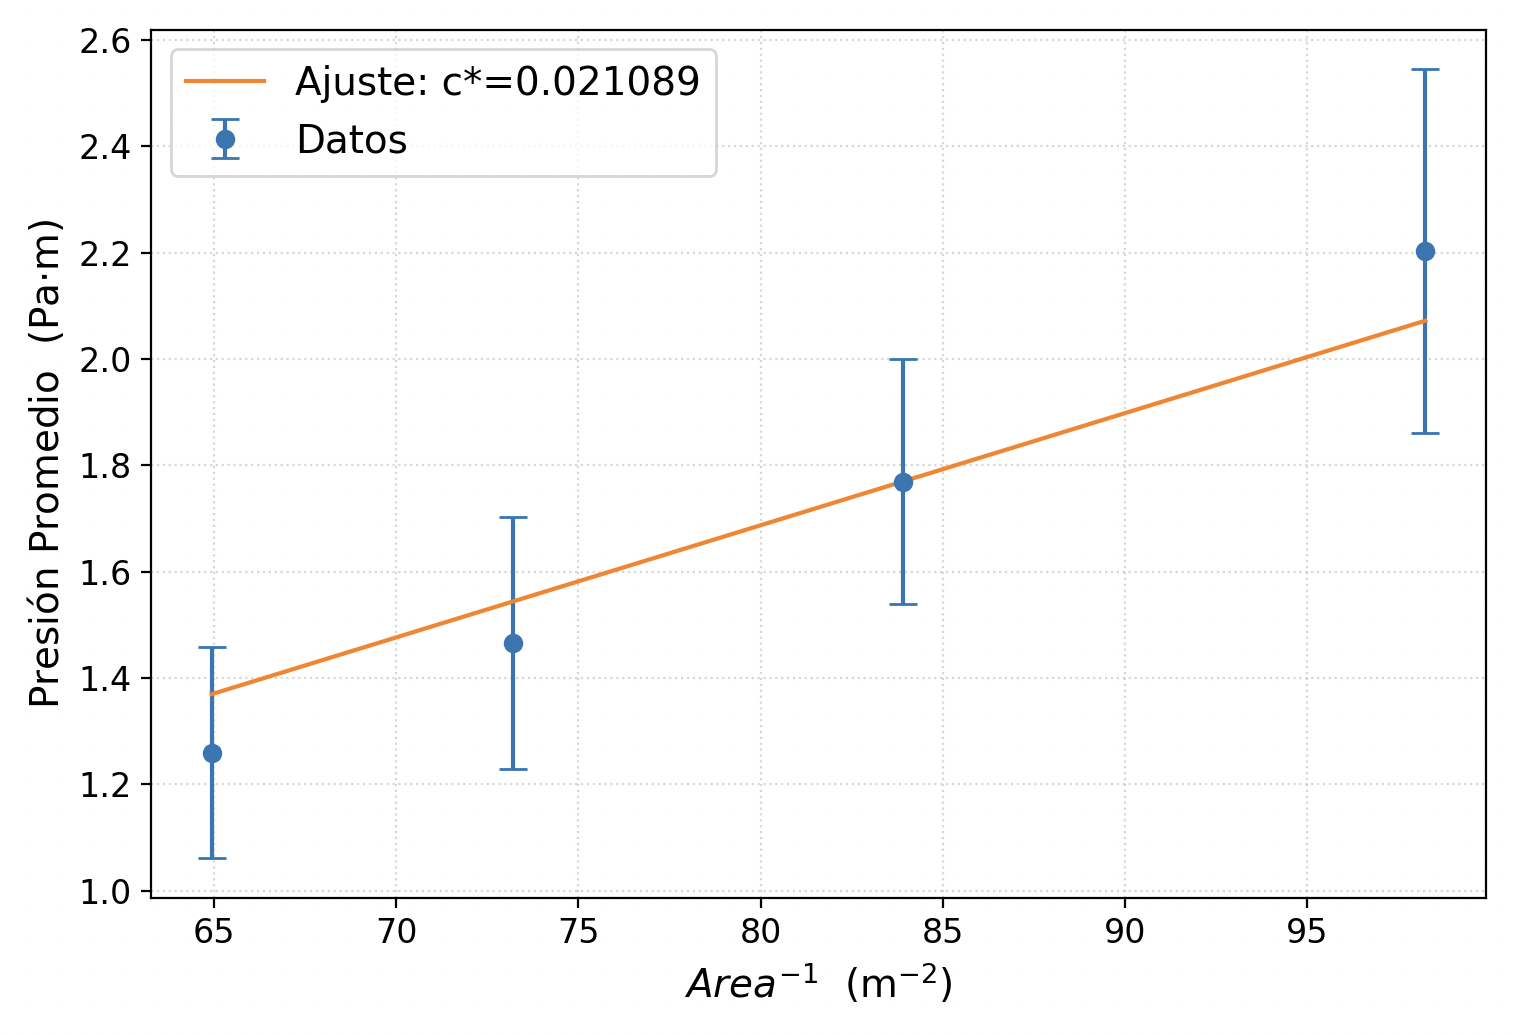
\includegraphics[width=\linewidth]{resources/regresion.png}
    \end{columns}
    \vspace{0.5cm}
    \begin{beamercolorbox}[sep=5pt,center]{block body}
        \begin{minipage}[t]{0.3\textwidth}
            \centering
            \small{$N=300$}
        \end{minipage}
        \hfill
        \begin{minipage}[t]{0.3\textwidth}
            \centering
            \small{$T=30\,000$}
        \end{minipage}
    \end{beamercolorbox}
\end{frame}

\begin{frame}{Cálculo del Coeficiente de Difusión}{Minimización del Parámetro de Ajuste}
    \begin{columns}[c]
        \column{0.60\textwidth}
            \centering
            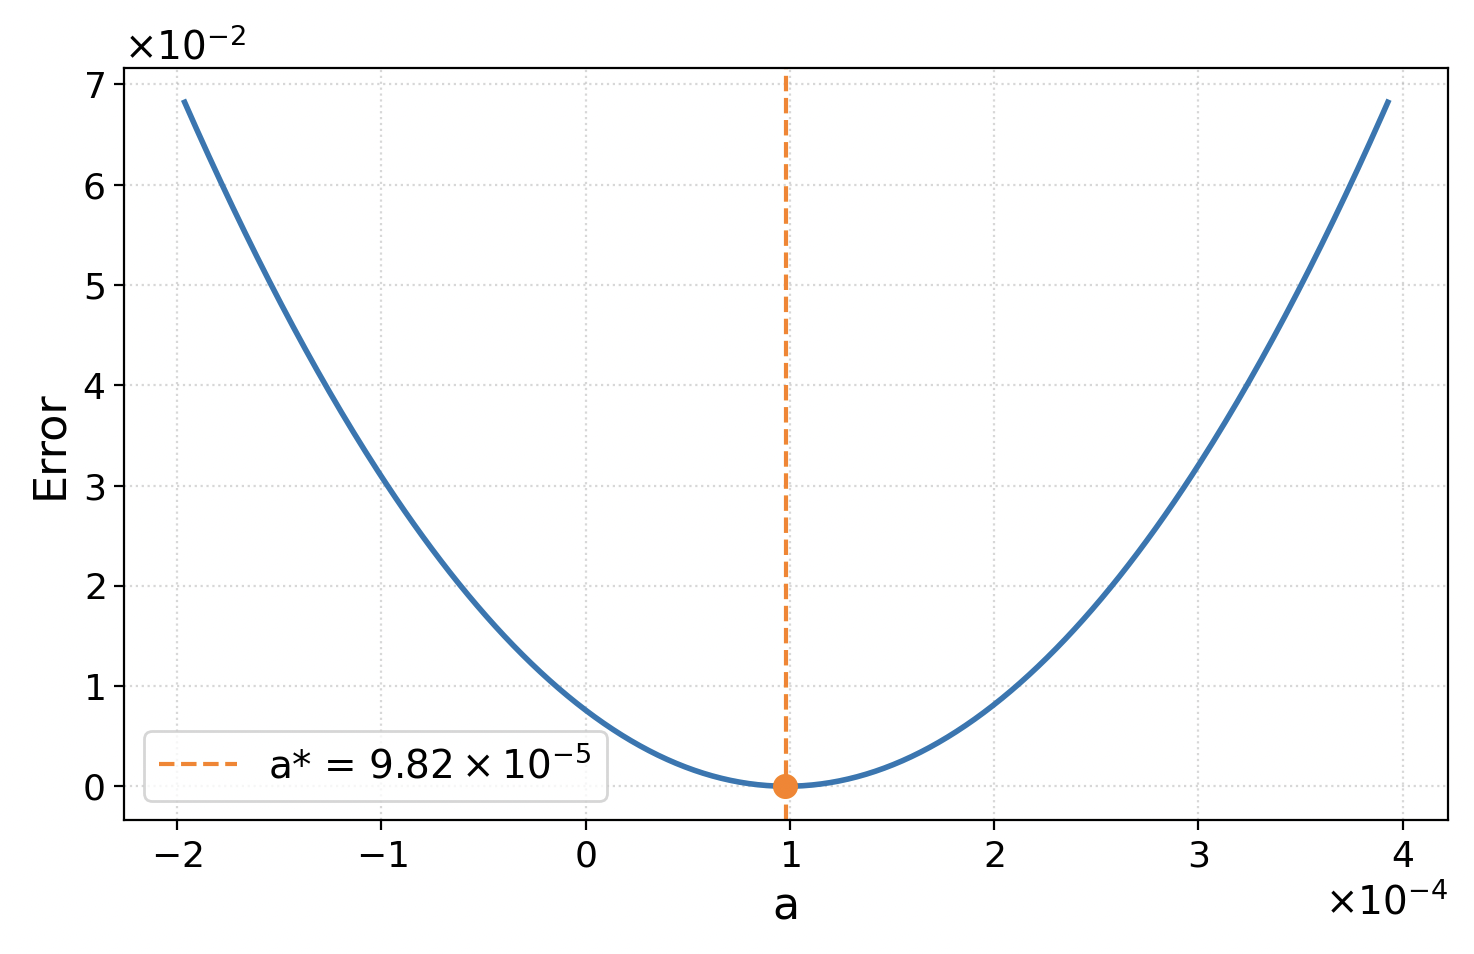
\includegraphics[height=.50\textheight]{resources/error-difusion.png}
        \column{0.40\textwidth}
            \begin{minipage}[t]{\linewidth}
                \begin{block}{Valores Tomados}
                    \begin{itemize}
                        \item $N=300$
                        \item $T=30\,000$
                        \item $L=0.09$m
                        \item $t_0=40$s
                    \end{itemize}
                \end{block}
            \end{minipage}
    \end{columns}
\end{frame}

\begin{frame}{Cálculo del Coeficiente de Difusión}{Graficó del MSD y Valor Obtenido}
    \begin{columns}[c]
        \column{0.60\textwidth}
            \centering
            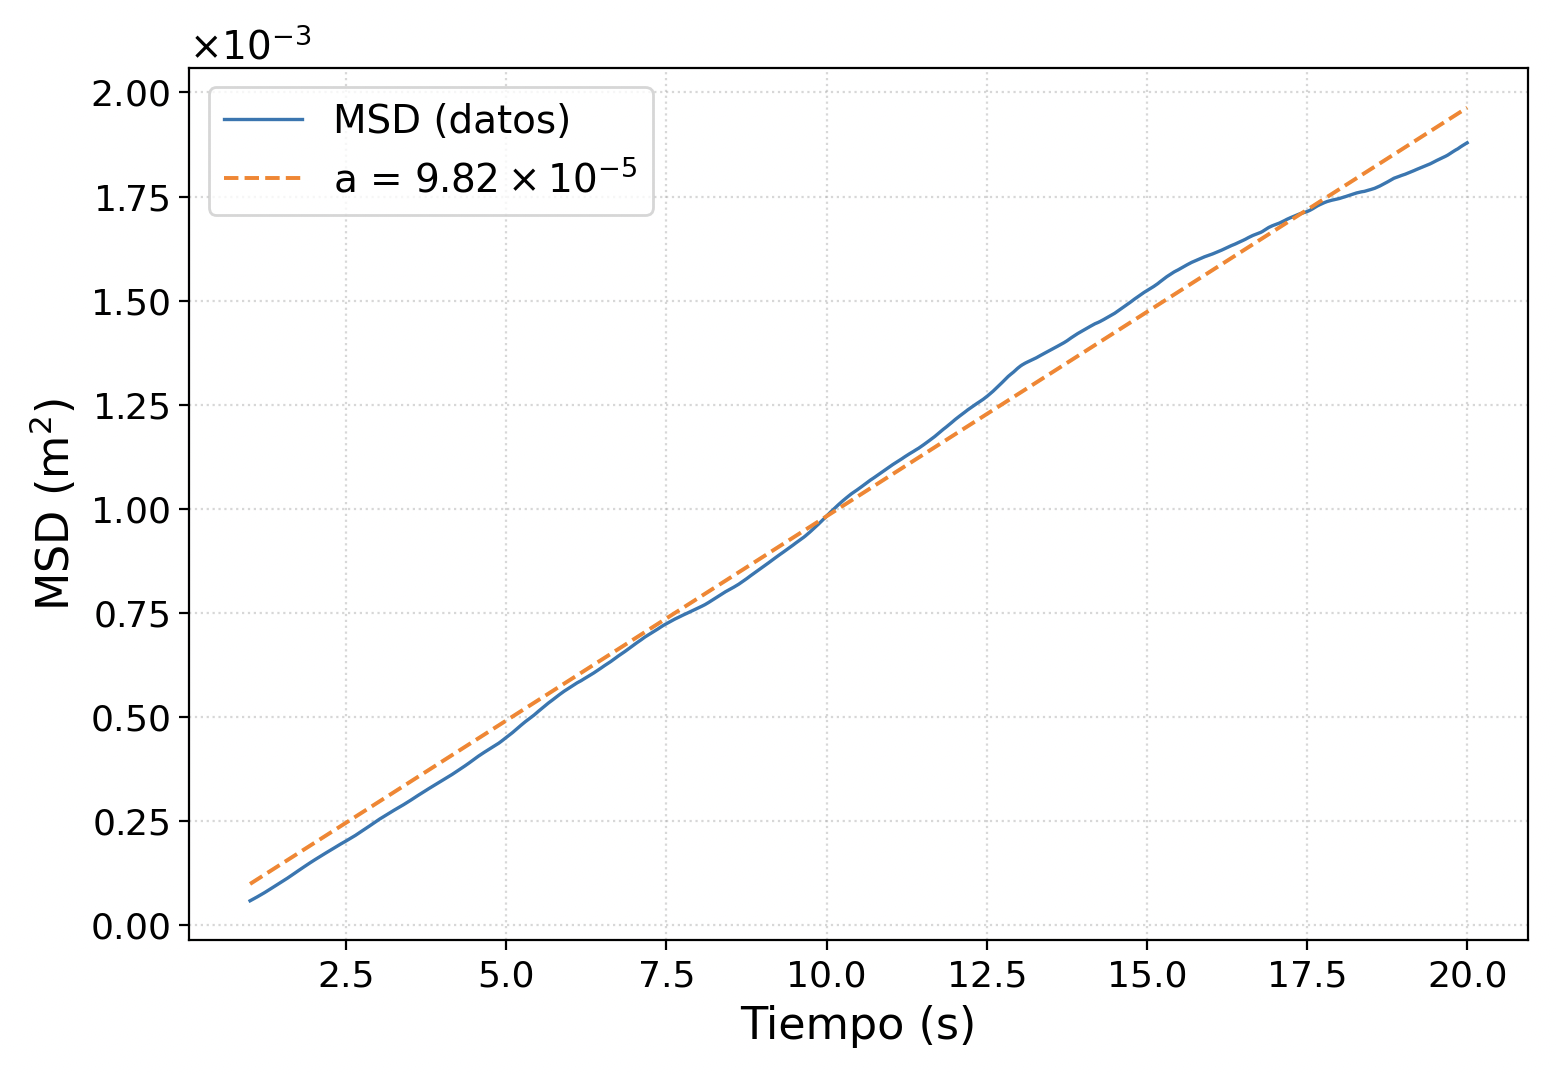
\includegraphics[height=.55\textheight]{resources/difusion.png}
        \column{0.40\textwidth}
            \begin{minipage}[t]{\linewidth}
                \begin{block}{Resultado}
                    \begin{itemize}
                        \item $D=2.46\cdot10^{-5}$m$^2$/s
                    \end{itemize}
                \end{block}
            \end{minipage}
    \end{columns}
\end{frame}

% Sección 5
\section{Conclusiones}
\begin{frame}{Conclusiones}
    \begin{itemize}
        \item La presión en ambos recintos converge a un valor estacionario.
        \item A mayor valor de $L$, hay un leve incremento en el tiempo para alcanzar el estaicionario.
        \item Tomando el régimen estacionario, la curva $\bar{P}$ vs $A^{-1}$ exhibe un comportamiento creciente que se aproxima a una relación lineal.
        \item El ajuste lineal con $c^*$ respalda la relación casi lineal de $\bar{P}$ en función de $A^{-1}$, lo que indica que el comportamiento se asemeja al de un gas ideal.
        \item El valor de $D$ se corresponde con la difusión de un gas.
    \end{itemize}
\end{frame}


\begin{frame}
    \begin{beamercolorbox}[sep=8pt,center]{title}
        \usebeamerfont{title} Muchas gracias
    \end{beamercolorbox}
\end{frame}
\end{document}
